% script to create a pdf document
% > latex howto.txt
% > dvipdf howto.dvi

\documentclass[12pt]{report}

% Default margins are too wide all the way around. I reset them here
\setlength{\topmargin}{-.5in}
\setlength{\textheight}{9in}
\setlength{\oddsidemargin}{.125in}
\setlength{\textwidth}{6.25in}

\usepackage{graphicx}

% Figures with borders
\usepackage{float}
\floatstyle{boxed} 
\restylefloat{figure}

\begin{document}
\title{MetiTree User Guide}
\author{
Michael van Vliet\\
Miquel Rojas Cherto}
\renewcommand{\today}{March 2012}

\maketitle

\newpage
This User Guide provides an overview of features of the MetiTree web application. Use 
the content list to enter detailed information on how to use MetiTree. 

\begin{center}
\begin{figure}[h!]	
%  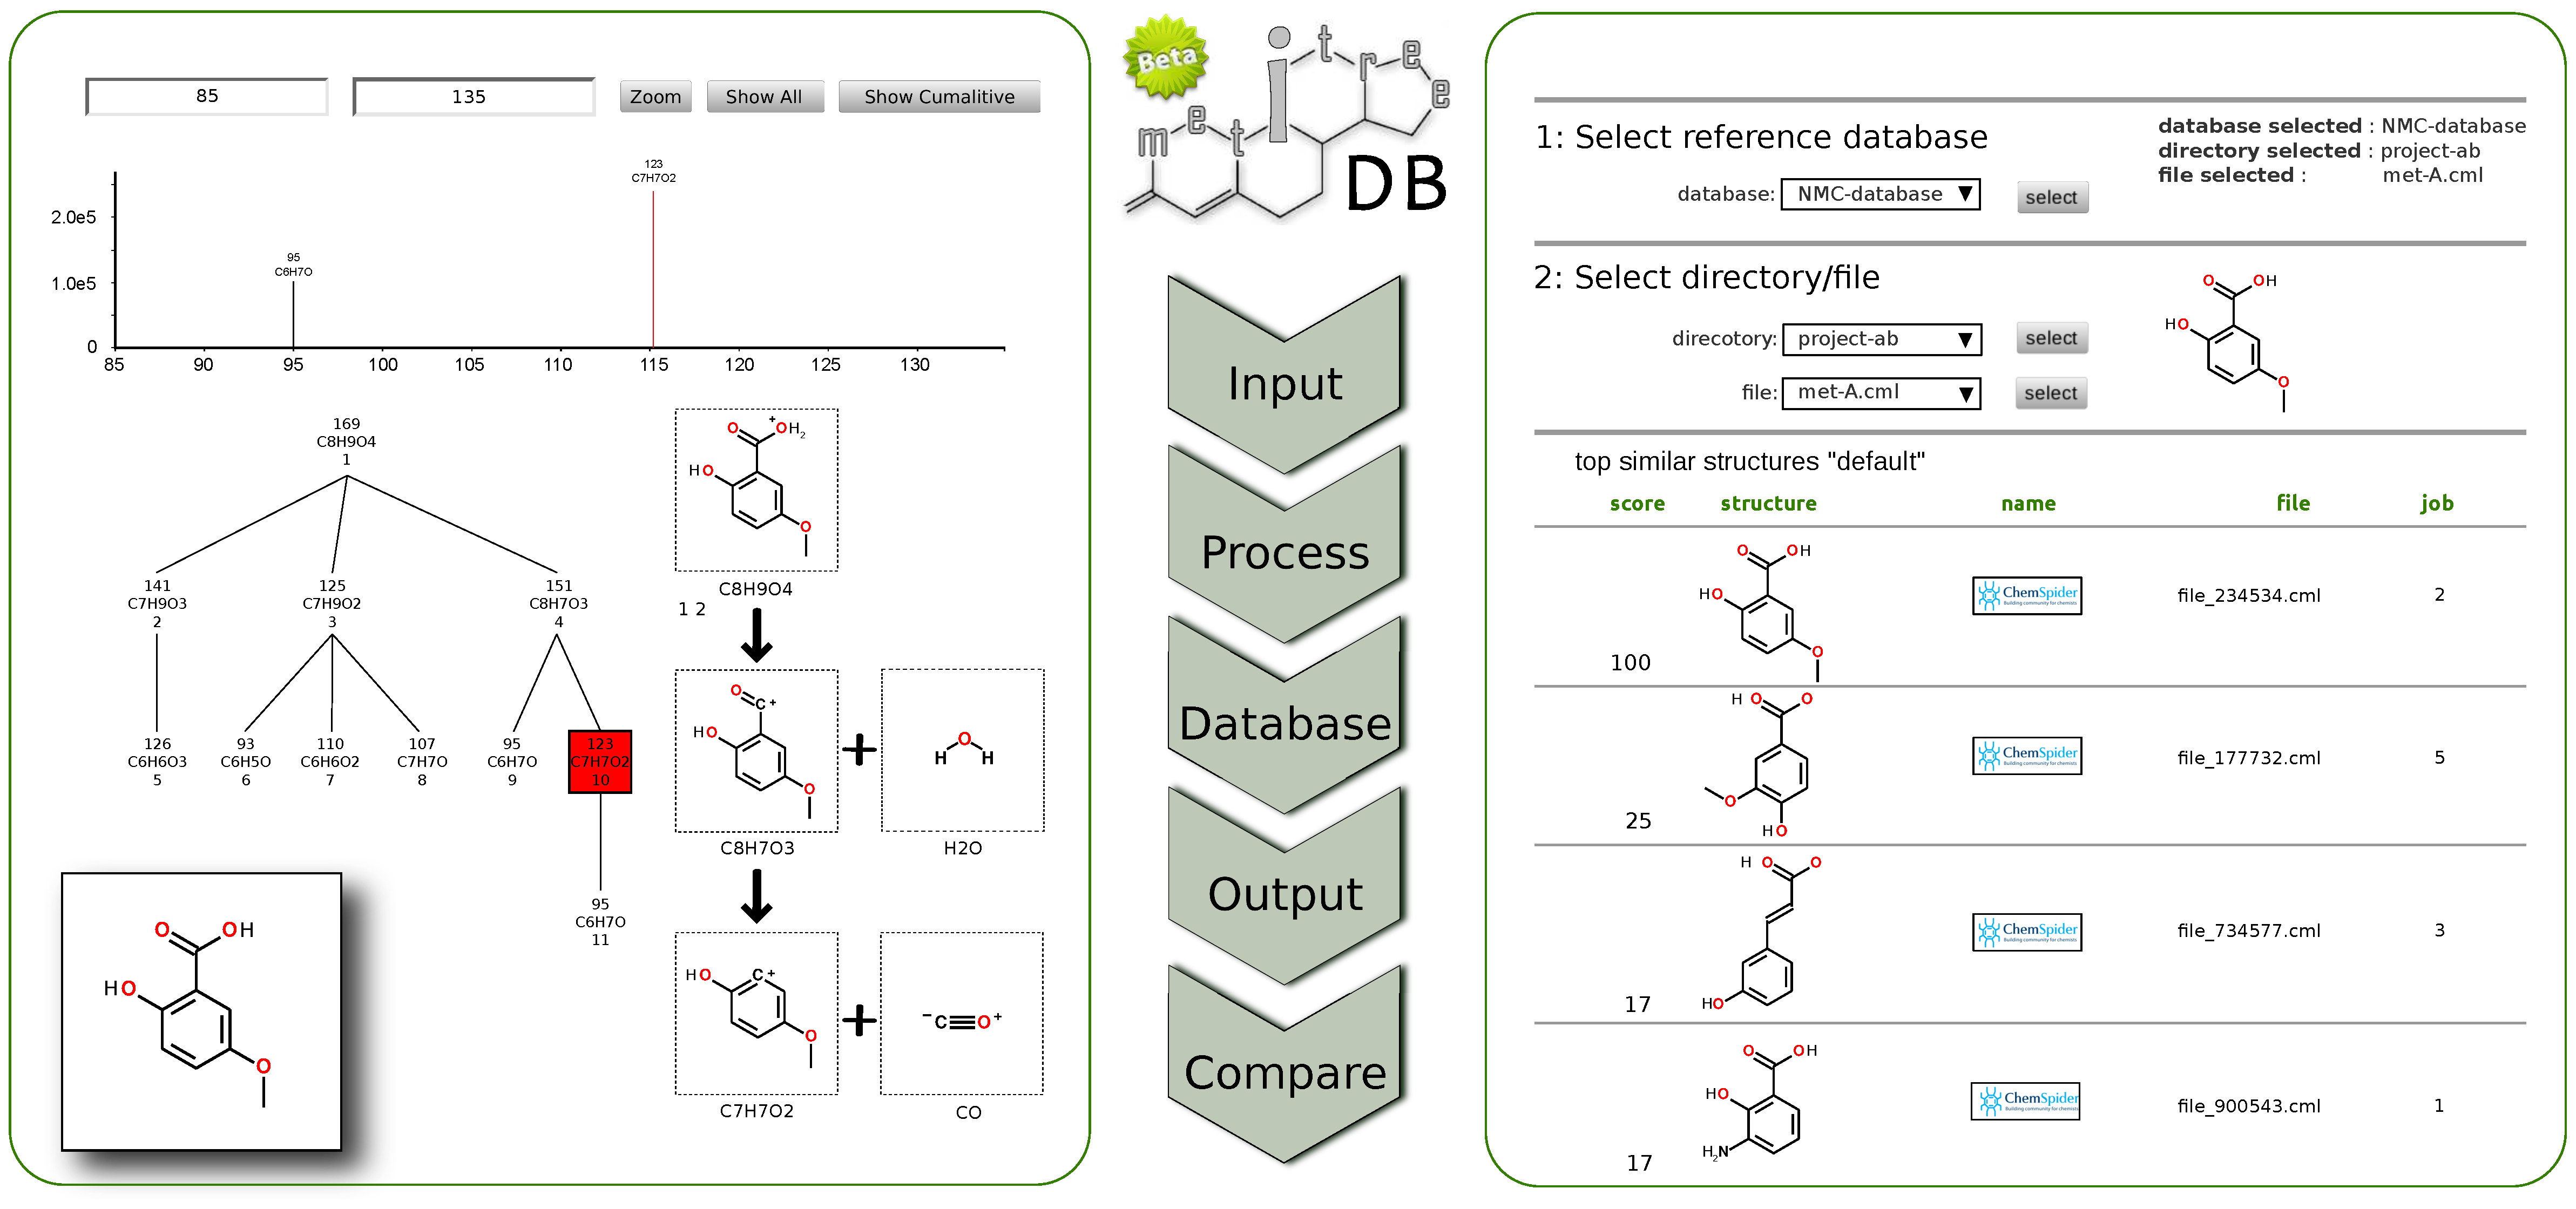
\includegraphics[scale=0.2]{metitreeSchema.eps}
\end{figure}
\end{center}


\section{MS$^n$ data}
\framebox[1.1\width]{Upload files with MSn mass spectrometry data and store them into data directories. } 
\newline

Metitree accept right now the uploading of mzXML files containing MSn mass spectrometry data. MetiTree creates directories for grouping mzXML files, assisting with the organization of the data according projects or topics. 

\begin{enumerate}

\item Log in as a user. 
\item Select "\textbf{MSn data}" (tap), to open the "\textbf{MSn data}" page.
\item The "\textbf{MSn data}" page will display. From this page, you can perform the functions listed below:
\begin{itemize}
    \item Create a new directory
    \item Modify an existing directory
\end{itemize}
\item To create new directory, provide a name for the new directory. Click "\textbf{create}" to save your directory.
			
\begin{center}
\begin{figure}[H]
%  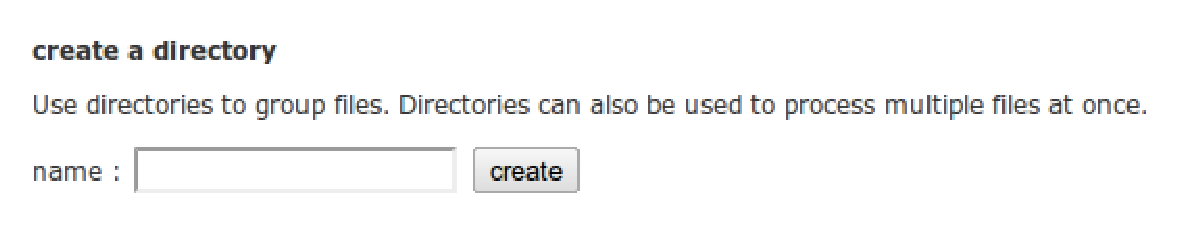
\includegraphics[scale=.8]{createDirectory.eps}
\end{figure}
\end{center}

\item To modify a existing directory, select one of the directories

\begin{center}
\begin{figure}[H]
%  \includegraphics[scale=.8]{a.eps}
\end{figure}
\end{center}

\item The page "\textbf{Files}" will be displayed. The files added into the
directory will be listed.

\item 7. Select "\textbf{Choose File}" to added new files from your
desktop to this directory. Finally, select "\textbf{submit}" to
save it.

You can upload a single mzXML file or a zip-file with multiple mzXML files.

\item Ones the file/s is uploaded you can introduce the InChI identifier of the
neutral compound. To save the InChI identifier you have to select the "\textbf{update}" button. Automatically, the file will be cross-related to the pubchem and chemspider database.
\item The files can be sorted by name or data created by selecting
"\textbf{name/date}".

\end{enumerate}

\newpage
\section{Process}
\framebox[1.1\width]{Process, visualize the results of MSn data.} 
\newline

The required input to process MSn data are mzXML files and the settings of the processing parameters. Processing parameters are grouped into those to extract the mass spectrometry information (m/z, intensity, and retention time) and those to enrich the MS data with chemical information (elements and number of atoms). MetiTree allows the processing of individual or multiple files at the same time. Furthermore, the same mzXML file can be processed several times with different sets of parameters. Results and parameters information are stored to allow for posterior revision.
 
Once the data is processed, it can be displayed using the spectral tree viewer. Here, the user can select a peak or a node, which represent a fragment. For each selection, the corresponding spectrum is displayed, together with the reactions that connect the parent ion with the selected fragment. The structure of the fragments is only visible when it has been assigned. The results generated by MetiTree can be exported to different formats (CSV, CML, and PDF) for further analysis. The CML, system for managing complex chemical content, which other software can import to process it even further. The PDF, format used to visually the MSn data, which makes suitable to export images into reports or publications. 

\begin{enumerate}
 
\item On the left navigation bar select "\textbf{Process}" (tap)
\item To process a files you must firstly to select the directory where is found
the file or files. To process all files of a determined directory select "\textbf{process directory}".

\begin{center}
\begin{figure}[H]
%  \includegraphics[scale=.8]{a.eps}
\end{figure}
\end{center}

\item If you want to specify specific files from the directory, select
"\textbf{select file(s) from directory to process}". A list of files will be
displayed. Check those files interested to process and select "\textbf{process files}"

\begin{center}
\begin{figure}[H]
%  \includegraphics[scale=.8]{a.eps}
\end{figure}
\end{center}

\item It will display the "\textbf{Define settings}" page.
Introduce the following settings:
\begin{itemize}
    \item MZ gap (bin size) = Bin size of a pick allowed during the peak picking extraction.
	\item Signal to noise threshold = Signal to noise threshold allowed during the
	peak picking extraction.
	Elements = It defines upper and lower number of atoms admitted for each element
in the elemental composition of the ion.
	Rules = It defines the constraint-rules that are applied to verify the
elemental compositions generated. It distinguish between the Nitrogen Rules and the RDB rules.
	Mass accuracy settings = Mass accuracy error allowed by MS level.
\end{itemize}

\begin{center}
\begin{figure}[H]
%  \includegraphics[scale=.8]{a.eps}
\end{figure}
\end{center}

\item To submit the process select "\textbf{Process}".

\begin{center}
\begin{figure}[H]
%  \includegraphics[scale=.8]{a.eps}
\end{figure}
\end{center}

\item The "\textbf{Process}" page will display.
\item It is possible to visualize the different results. Between them you have:
\begin{itemize}
    \item xcms = output generated by XCMS after the peak picking extraction.
	\item cml = chemical markup language file enriched with chemical information.
	\item trees = Tree Viewer interconnects three MSn items: the spectrum, which
contains mass peaks, the fragmentation tree, which contains fragment nodes/elemental compositions, and the fragmentation reactions, which contain structures.
	\item master tree = A viewer that filters the tree file based on the occurrence
of each fragment.
	\item csv = comma separated values file with enriched chemical information
	\item pdf = portable document format to visualize the spectral data.
\end{itemize}

\item Select “master tree” to visualize spectral data with the tree viewer

\begin{center}
\begin{figure}[H]
%  \includegraphics[scale=.8]{a.eps}
\end{figure}
\end{center}
\end{enumerate}
 
\newpage
\section{Storage}
\framebox[1.1\width]{Manage database(s) with MSn data.} 
\newline

Processed MSn data can be stored in one or multiple internal databases. Because the users are organized in groups, they can share files and libraries with other group members. All MSn data can be labeled with an InChI identifier of the compound that is automatically cross referenced with PubChem and ChemSpider databases. 

\begin{enumerate}
 
\item On the left navigation bar select "\textbf{Databases}" (tap)
\item The "\textbf{Databases}" page will display. From this page, you can perform the functions listed below:
\begin{itemize}
    \item Create a new database
    \item Modify an existing database
\end{itemize}
\item To create new database, provide a name for the new database. Click
"\textbf{add}" to save your database.

\begin{center}
\begin{figure}[H]
%  \includegraphics[scale=.8]{a.eps}
\end{figure}
\end{center}

\item To modify a existing database, select one of the databases 

\begin{center}
\begin{figure}[H]
%  \includegraphics[scale=.8]{a.eps}
\end{figure}
\end{center}

\item Modify the files to be contained in the database as required.

\begin{center}
\begin{figure}[H]
%  \includegraphics[scale=.8]{a.eps}
\end{figure}
\end{center}

\item On the right side you have the files that actually are contained in the
database. On the left side you have those files that you can upload to the
database. Through "\textbf{filter on job}" you can filter the files by specific job.

\end{enumerate}

\newpage
\section{Data search}
\framebox[1.1\width]{Query in an existing database(s) similar MSn data. } 
\newline

MetiTree integrates the functionality to query for similar MSn data stored in your personal library. The results are presented in a list showing the structures of the most similar MSn data together with the corresponding similarity value. The results are ranged between 0-100. Value near to 100 indicates that MSn data is highly similar; while a value close to 0 illustrates that it is very different. We expect MetiTree to contribute two fold in the identification of metabolites. On one hand, we are interested to know if a fragmentation tree of the same compound is present in the library, which would be a partial identification. On the other hand, if similar fragmentation data is found, we can use this knowledge to give hints (e.g. substructure information) which structure the unknown compound could have. 

\begin{enumerate}
\item Log in as a user.
\item Select "\textbf{search/compare}" (tap), to open the
"\textbf{database search}" page.
\item Choose a database to query "\textbf{database}", and the
spectral tree file to be compared in "\textbf{directory}" $>$
"\textbf{file}".

\begin{center}
\begin{figure}[H]
%  \includegraphics[scale=.8]{a.eps}
\end{figure}
\end{center}

\item The "\textbf{database search}" page will display the results
into a list of compound ranked from more similar to a less similar. In the left side it will shows the similarity value when the fragmentation trees are compare each other.

\begin{center}
\begin{figure}[H]
%  \includegraphics[scale=.8]{a.eps}
\end{figure}
\end{center}

\end{enumerate}

\newpage
\section{Visualize enriched MSn data}
Spectral tree viewer is capable to show the chemical structure of the fragments in the MSn data. At the moment it is only possible if you supply a JSON message describing the MSn data.


\begin{enumerate}
\item Log in as a user.
\item On the bottom, select the "\textbf{MsnViewer Demo}".
\item You can upload an example by selecting "\textbf{Load example}" >
"\textbf{view}".

You can modify the json message and add your own values. 

\begin{center}
\begin{figure}[H]
%  \includegraphics[scale=.8]{a.eps}
\end{figure}
\end{center}

\item After the selected view run, the MSn viewer screen will be shown.

\end{enumerate}

\newpage
\section{FAQ} 

\begin{itemize}
\item Where can I address for more help? 

For any questions that could not be answered through this guide, you can send us an email directly toinfo@metitree.nl. We will answer you promptly. 

\item Can I maintain my data permanently in Metitree? 

Due to Metitree is in a beta version every night all uploaded data or processed data is removed from the server. We expect that in the new release we will provide a persistent application. 

\item How many files might I upload to process?

At the moment you can only upload X number of files. We must limit with a small number to avoid collapsing our server.

\end{itemize}
\end{document}

